\documentclass[11pt,letterpaper]{article}
\usepackage{papernote}

\graphicspath{{serbin2012_photosynth/}}

\begin{document}

\papertitle{paper_title.png}

\begin{itemize}\setlength{\itemsep}{0.6em}
  \item \paperdoi{10.1093/jxb/err294}
  \item PLSR with full range spectrometers on leaves of trembling aspen and
        eastern cottonwood trees grown across an array of glasshouse
        temperature regimes.
  \item The wavelengths selected were correlated with known absorption
        features related to leaf water content, nitrogen concentration,
        internal structure, and/or photosynthetic enzymes.
  \item 13 wavelengths identified for Vcmax and 44 wavelengths for Jmax
        (Figure~\ref{fig:waves}).
\end{itemize}

\clearpage

\begin{figure}[H]
\centering
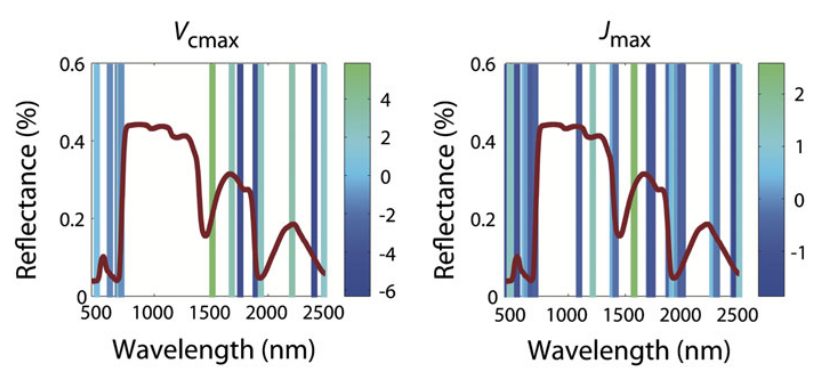
\includegraphics[width=0.95\textwidth]{waves_plot.png}\\[6pt]
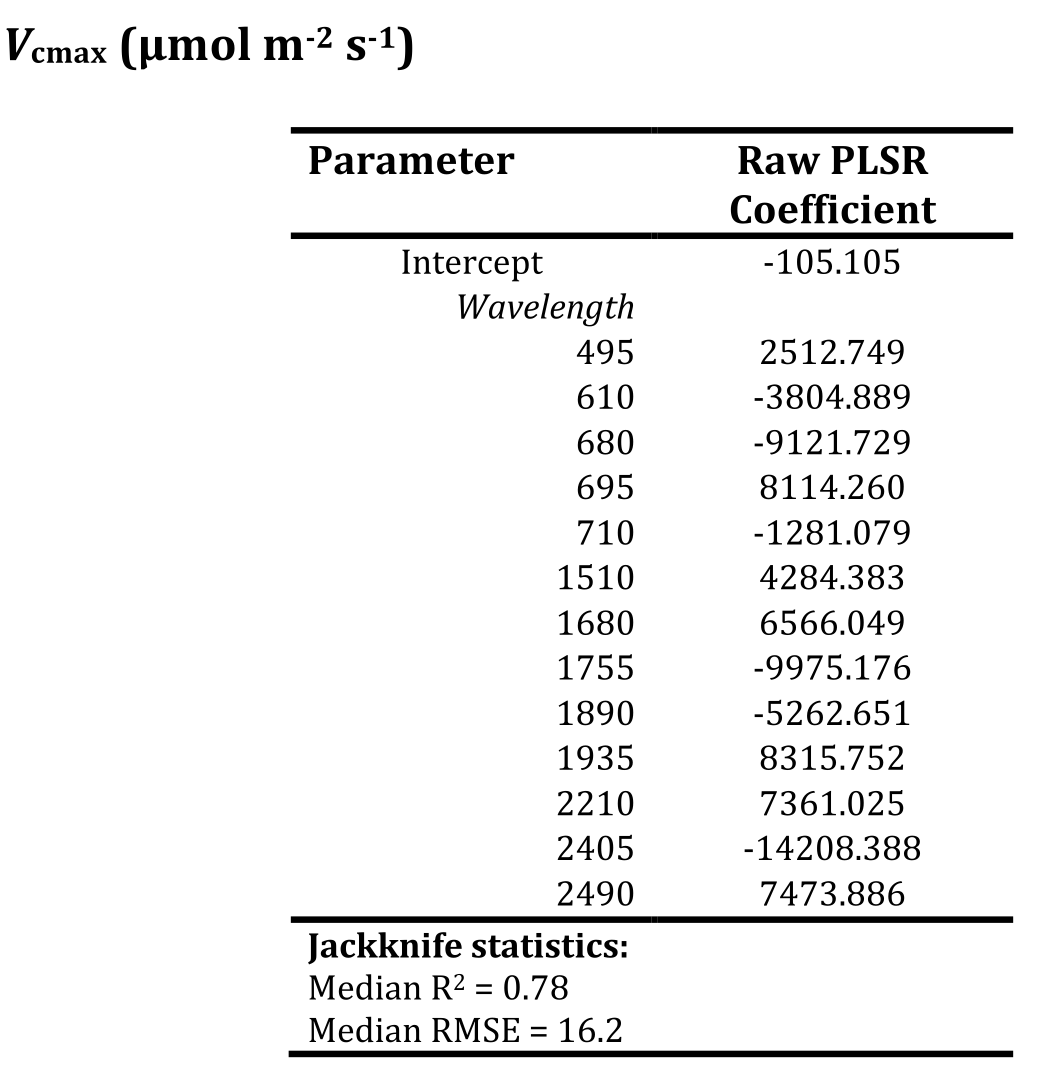
\includegraphics[height=4.5in]{vcmax_waves.png}\hfill
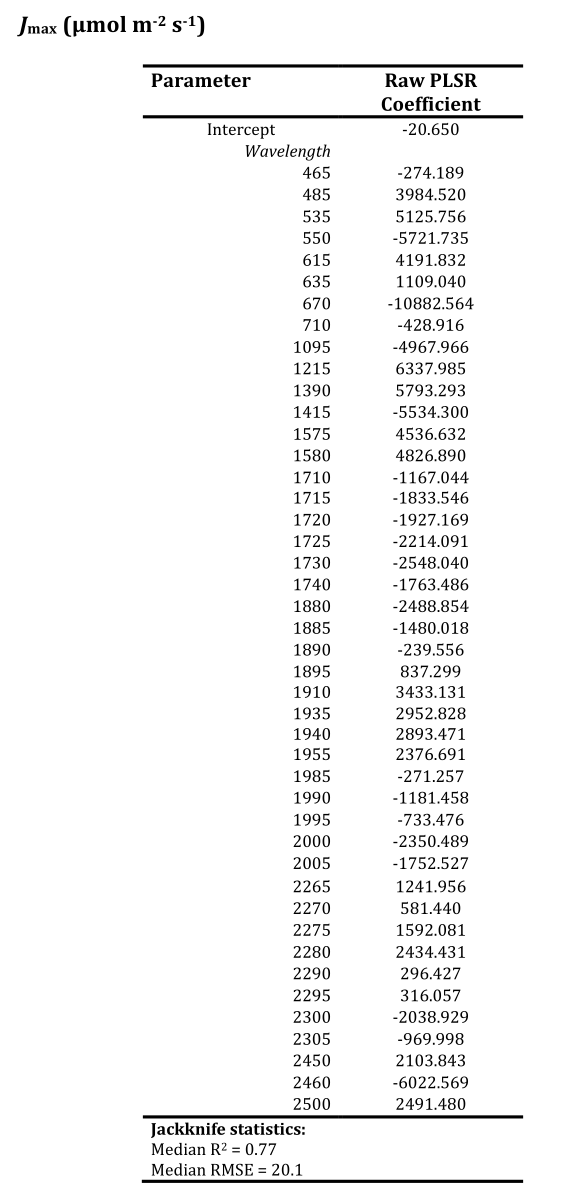
\includegraphics[height=4.5in]{jmax_waves.png}
\caption{Selected wavelengths for $V_\mathrm{cmax}$ and $J_\mathrm{max}$
PLSR models (top), and their raw PLSR coefficients (bottom). The
coefficient tables are from the SI of the paper.}
\label{fig:waves}
\end{figure}

\end{document}
